\chapter{DNS (Domain Name System)}\label{dns-domain-name-system}

\section{The Purpose of DNS}\label{the-purpose-of-dns}

\begin{itemize}
\tightlist
\item
  DNS is used to \emph{resolve} human-readable names (google.com) to IP
  ADDRESSES
\item
  Machines such as PCs don't use names, they use ADDRESSES (ie:
  IPv4/IPv6)
\item
  Names are much easier for us to use and remember than IP ADDRESSES

  \begin{itemize}
  \tightlist
  \item
    What is the IP ADDRESS of \href{http://youtube.com}{youtube.com} ?
  \end{itemize}
\item
  When you type `youtube.com` into a web browser, your device will ask a
  DNS SERVER for the IP ADDRESS of
  \href{http://youtube.com}{youtube.com}
\item
  The DNS SERVER(S) your DEVICE uses can be manually configured or
  learned via DHCP
\end{itemize}

\section{Basic Functions of DNS}\label{basic-functions-of-dns}

\begin{figure}
\centering
\pandocbounded{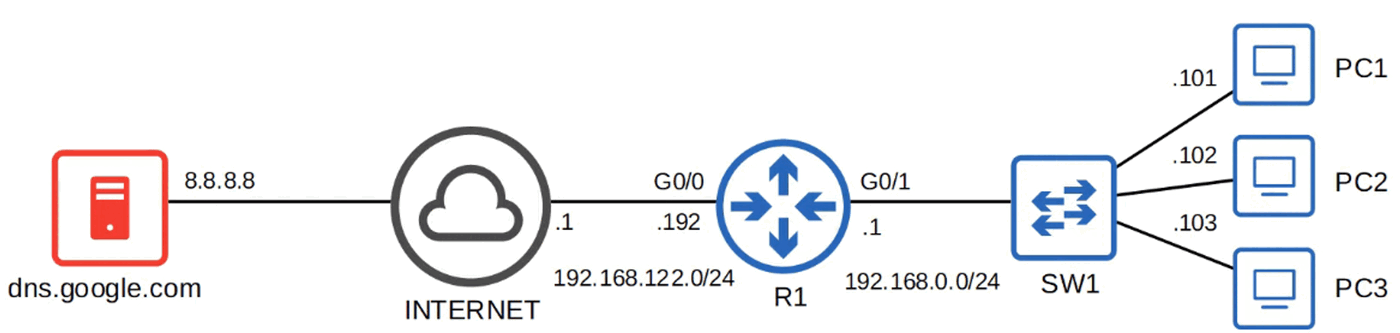
\includegraphics[keepaspectratio,alt={image}]{images/39-dns/img-001.png}}
\end{figure}

Command \passthrough{\lstinline!ipconfig /all!} (Show local IP
configuration on current DEVICE)

\begin{figure}
\centering
\pandocbounded{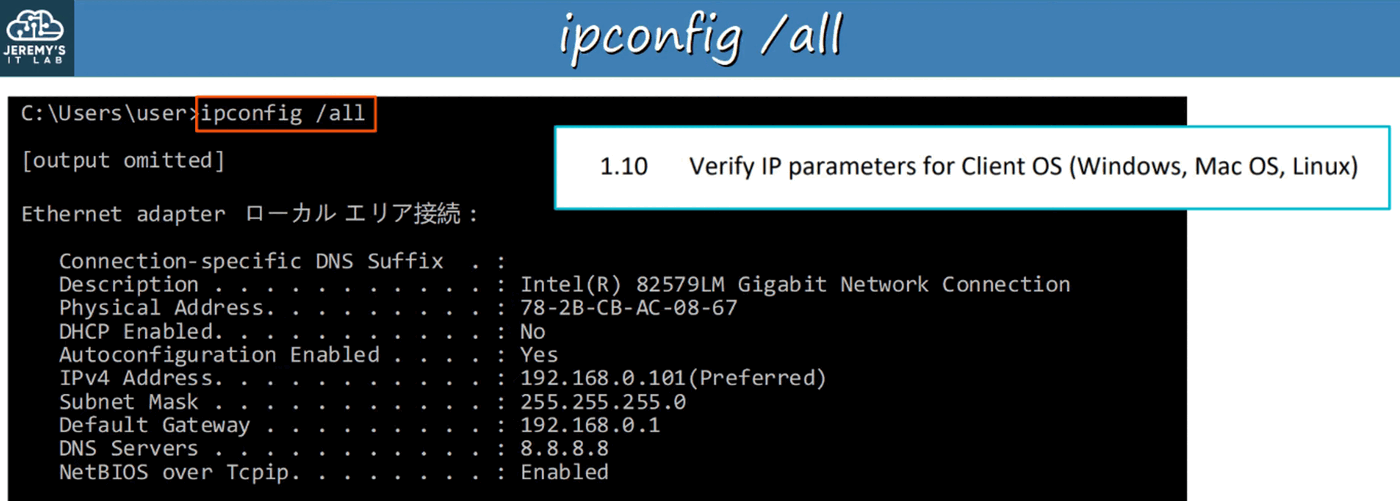
\includegraphics[keepaspectratio,alt={image}]{images/39-dns/img-002.png}}
\end{figure}

\begin{figure}
\centering
\pandocbounded{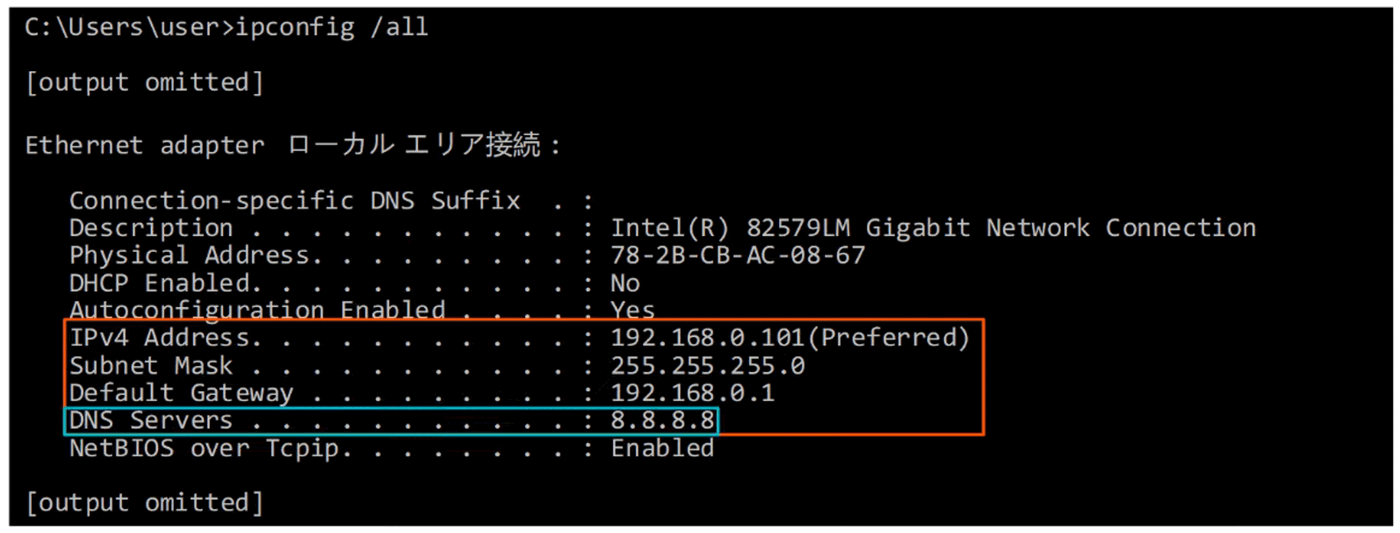
\includegraphics[keepaspectratio,alt={image}]{images/39-dns/img-003.png}}
\end{figure}

Command \passthrough{\lstinline!nslookup!} (Shows IP information for a
given DNS entry)

\begin{figure}
\centering
\pandocbounded{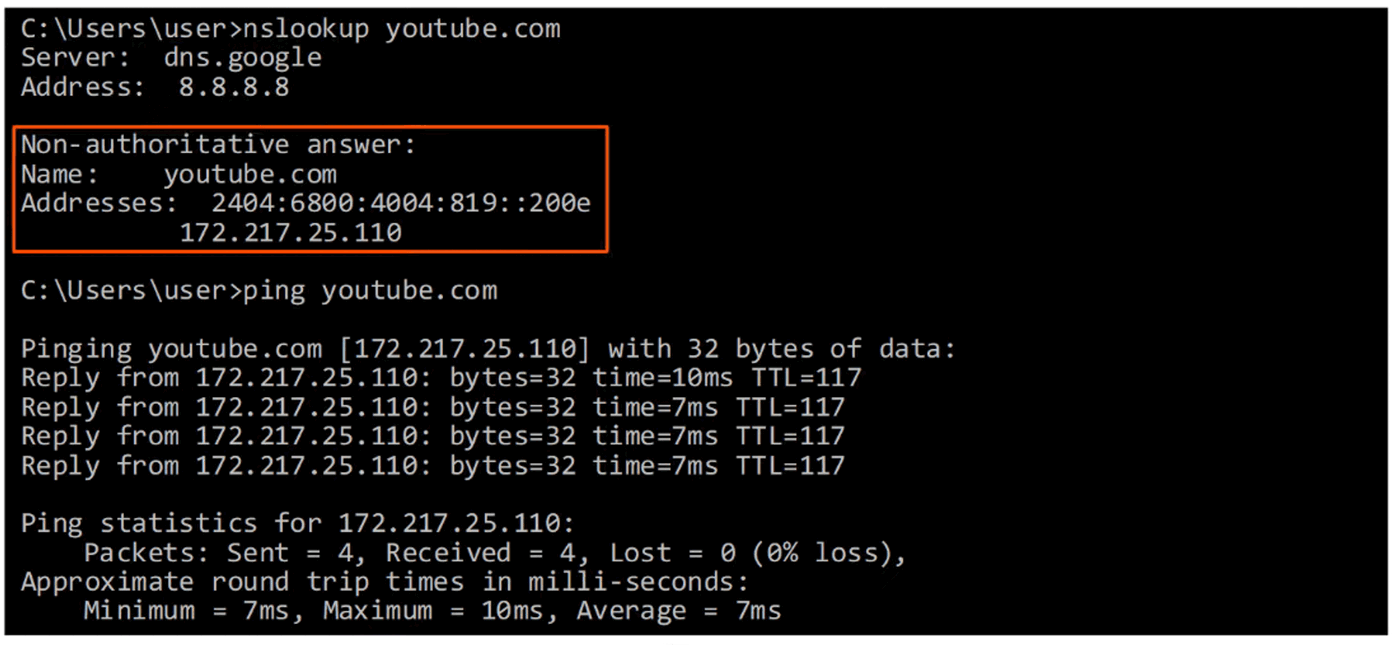
\includegraphics[keepaspectratio,alt={image}]{images/39-dns/img-004.png}}
\end{figure}

WIRESHARK CAPTURE of above COMMANDS

\begin{figure}
\centering
\pandocbounded{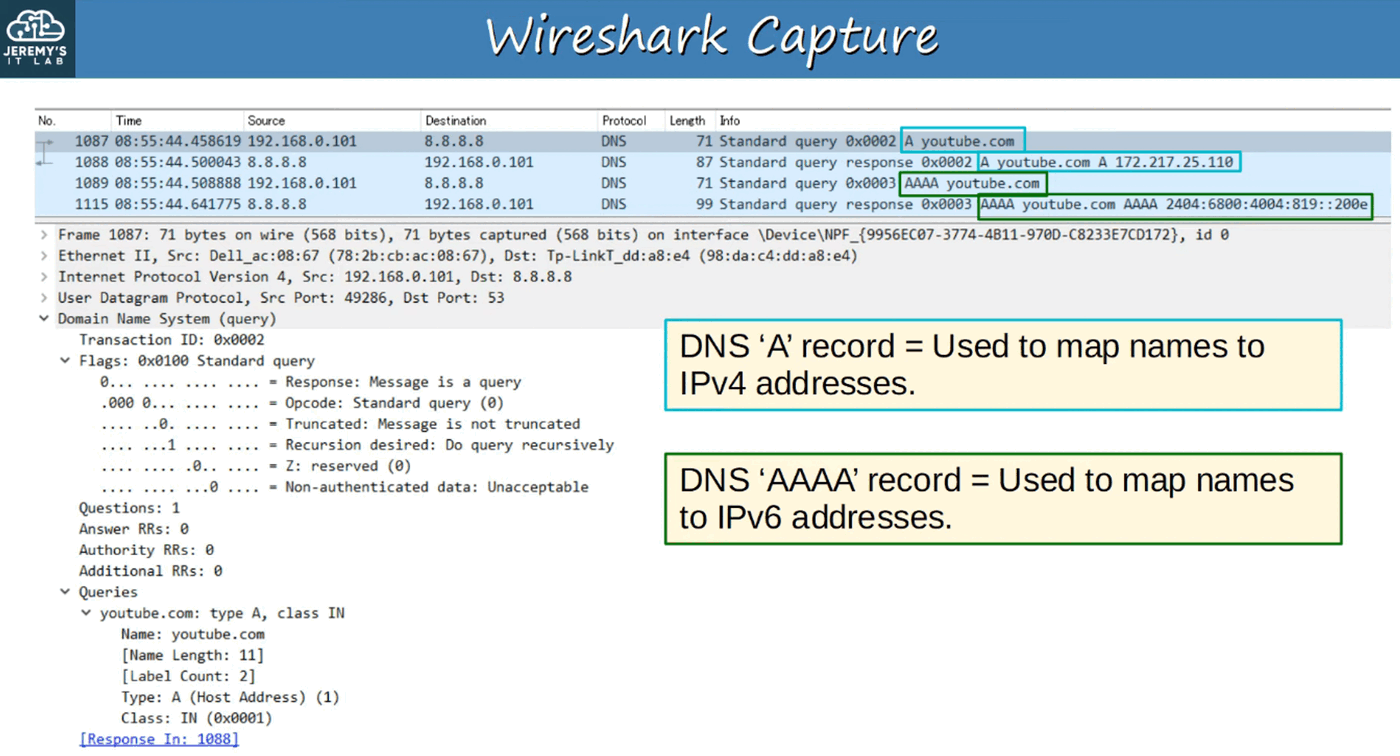
\includegraphics[keepaspectratio,alt={image}]{images/39-dns/img-005.png}}
\end{figure}

\begin{figure}
\centering
\pandocbounded{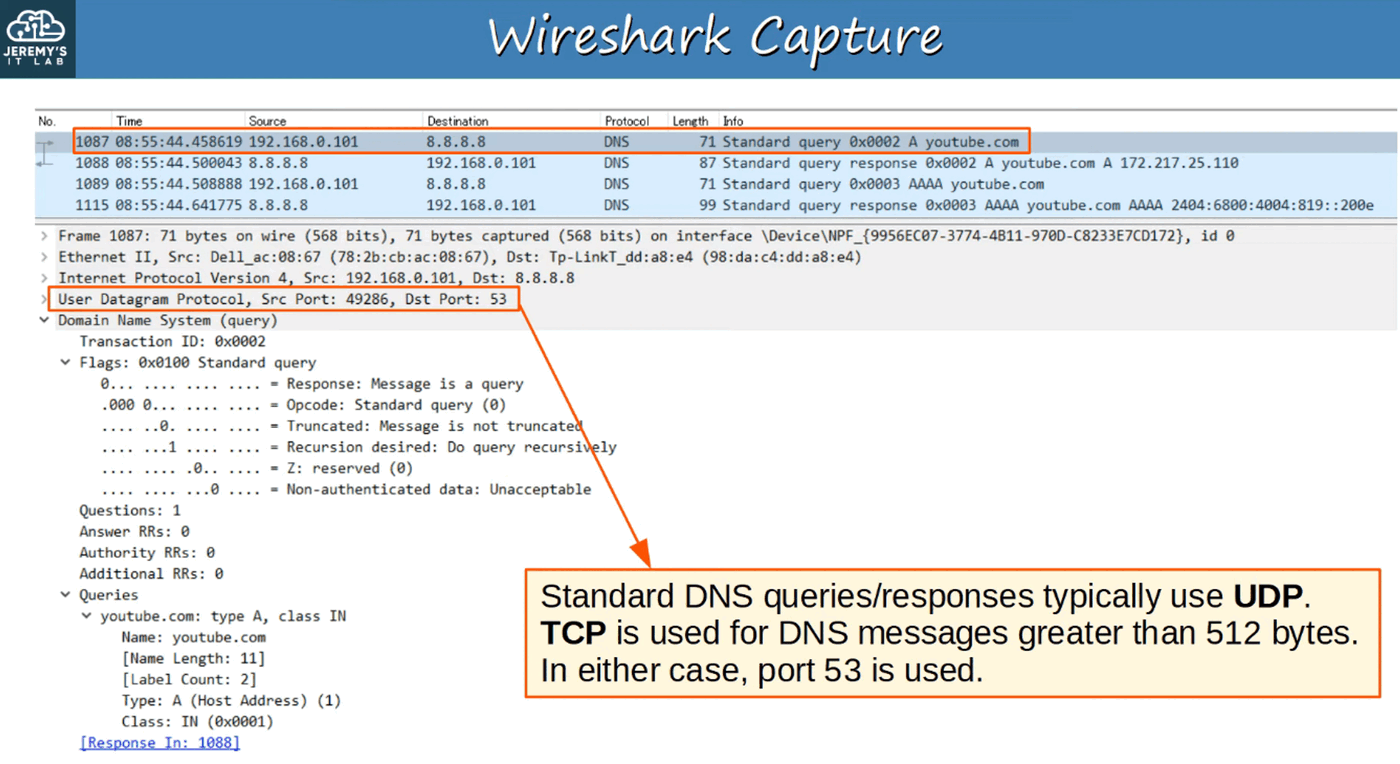
\includegraphics[keepaspectratio,alt={image}]{images/39-dns/img-006.png}}
\end{figure}

Command \passthrough{\lstinline!ipconfig /displaydns!} (Displays DNS
cache)

\begin{figure}
\centering
\pandocbounded{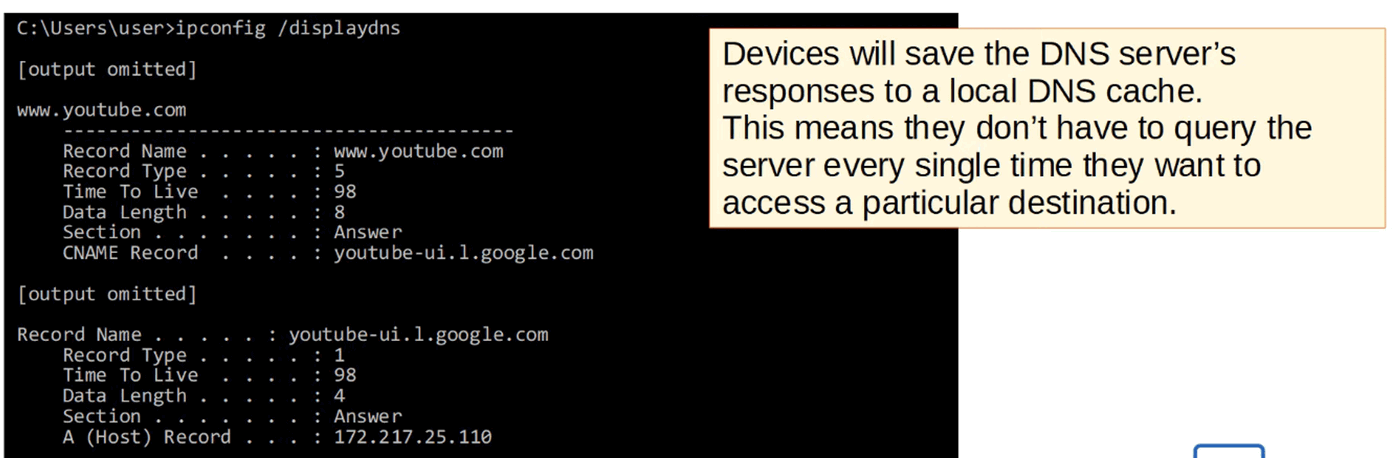
\includegraphics[keepaspectratio,alt={image}]{images/39-dns/img-007.png}}
\end{figure}

Command \passthrough{\lstinline!ipconfig /flushdns!} (Clears DNS cache)

\begin{figure}
\centering
\pandocbounded{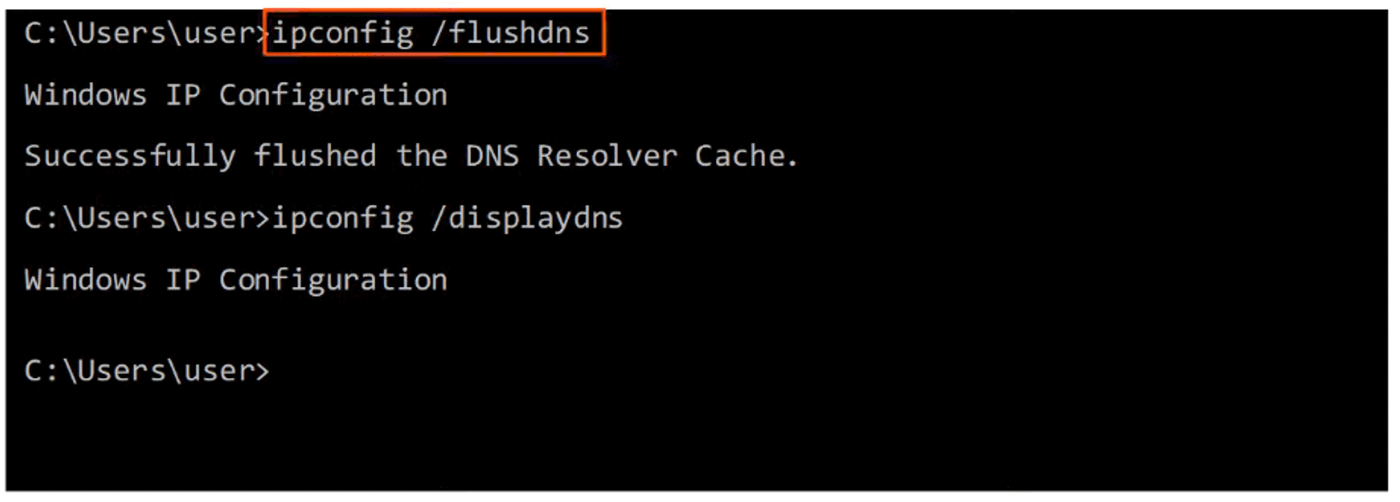
\includegraphics[keepaspectratio,alt={image}]{images/39-dns/img-008.png}}
\end{figure}

HOSTS Files

WINDOWS HOSTS location

\begin{figure}
\centering
\pandocbounded{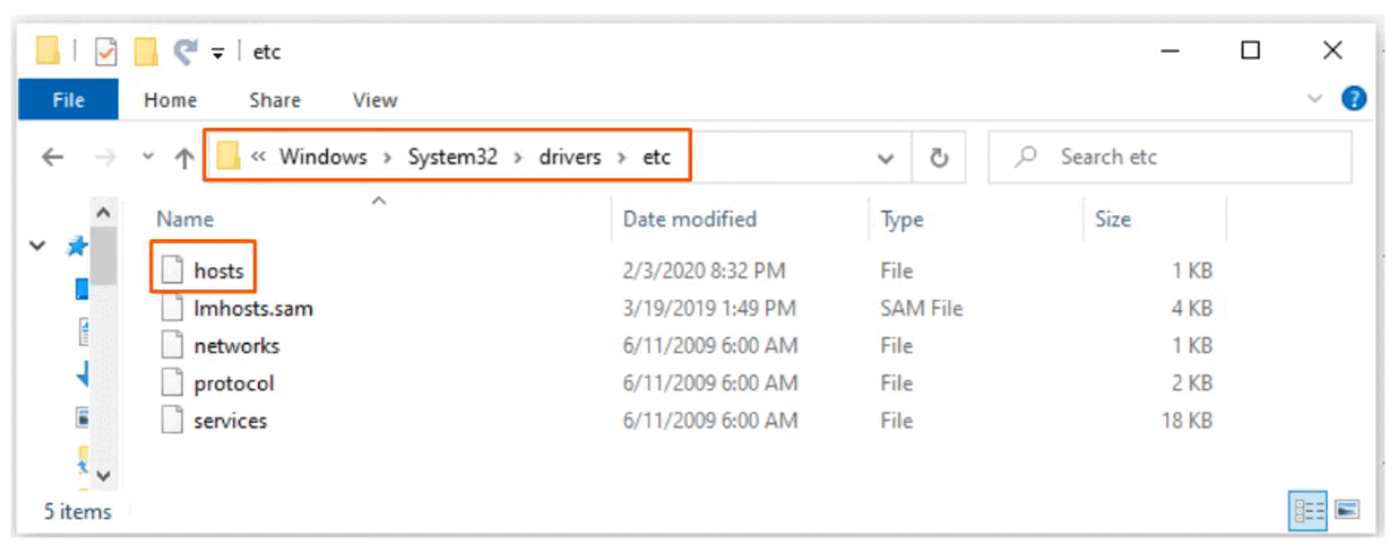
\includegraphics[keepaspectratio,alt={image}]{images/39-dns/img-009.png}}
\end{figure}

\begin{figure}
\centering
\pandocbounded{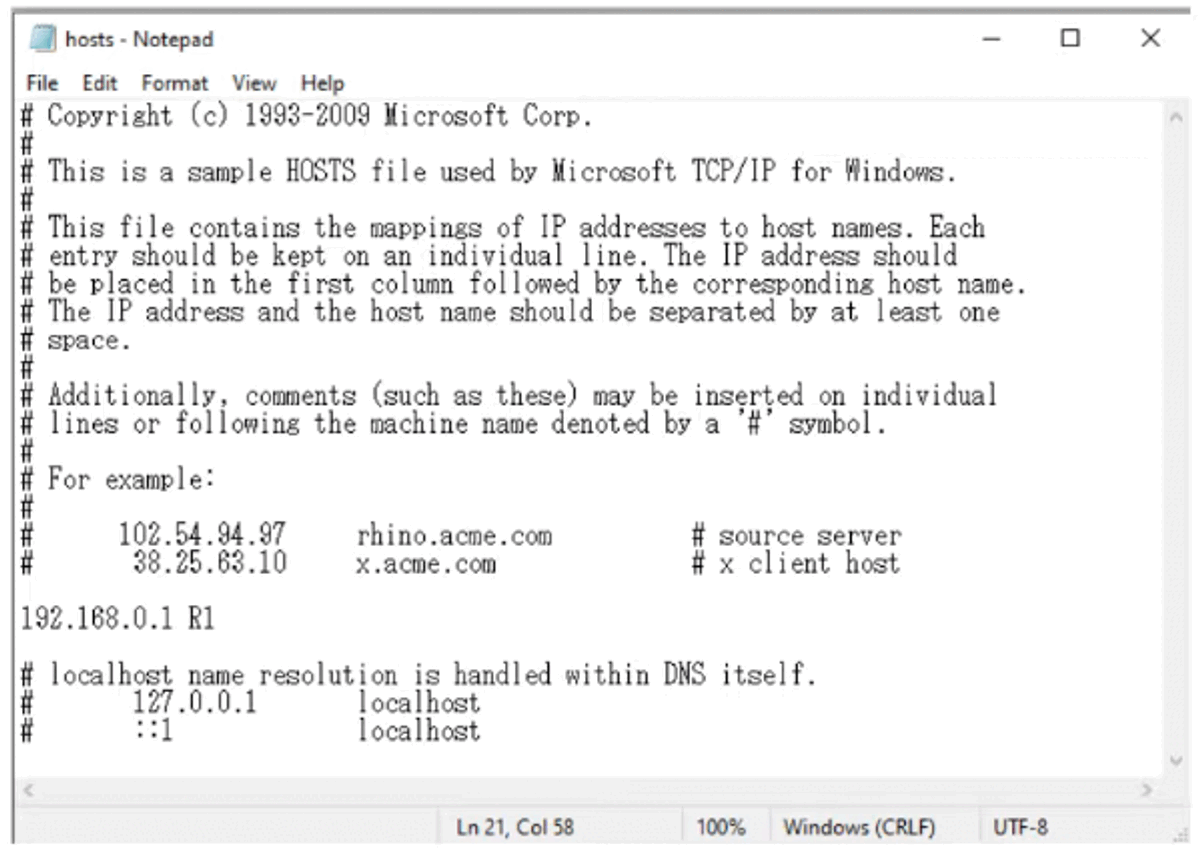
\includegraphics[keepaspectratio,alt={image}]{images/39-dns/img-010.png}}
\end{figure}

\section{Configuring DNS in Cisco
IOS}\label{configuring-dns-in-cisco-ios}

\begin{itemize}
\tightlist
\item
  For HOSTS in a NETWORK to use DNS, you don't need to configure DNS on
  the ROUTERS.

  \begin{itemize}
  \tightlist
  \item
    They will simply FORWARD the DNS messages like any other packets
  \end{itemize}
\item
  However, a CISCO ROUTER can be configured as a DNS SERVER, although
  it's rare

  \begin{itemize}
  \tightlist
  \item
    If an INTERNAL DNS SERVER is used, usually it's a WINDOWS or LINUX
    SERVER
  \end{itemize}
\item
  A CISCO ROUTER can also be configured as a DNS CLIENT
\end{itemize}

Command \passthrough{\lstinline!ip dns server!} and
\passthrough{\lstinline!ip host <hostname> <ip address>!}

\begin{figure}
\centering
\pandocbounded{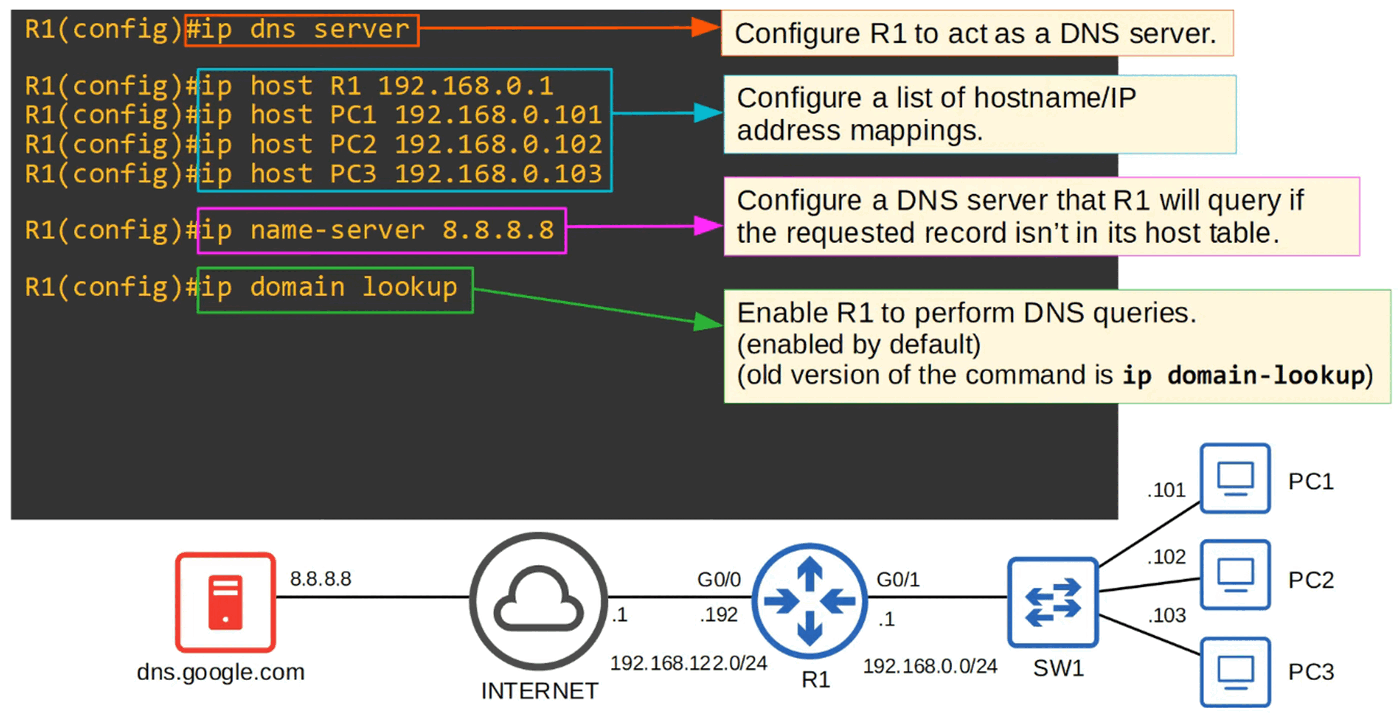
\includegraphics[keepaspectratio,alt={image}]{images/39-dns/img-011.png}}
\end{figure}

\begin{figure}
\centering
\pandocbounded{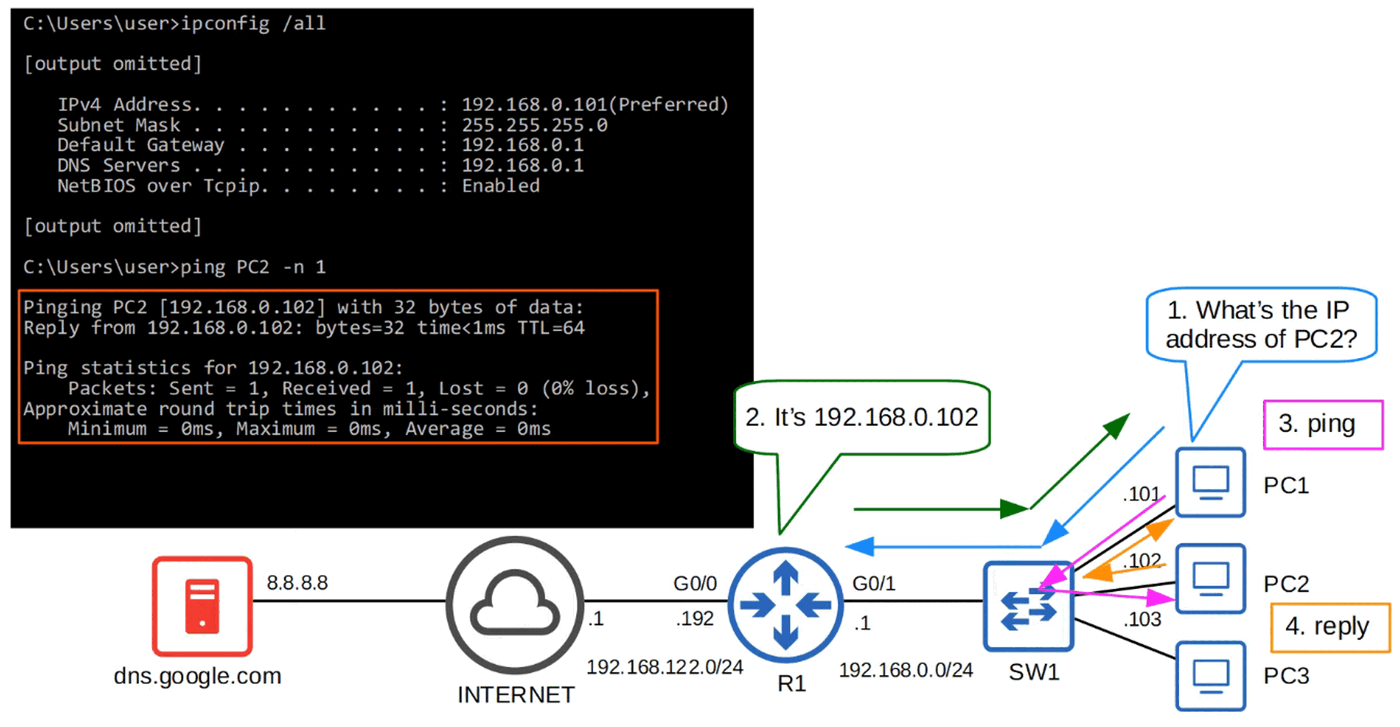
\includegraphics[keepaspectratio,alt={image}]{images/39-dns/img-012.png}}
\end{figure}

\begin{figure}
\centering
\pandocbounded{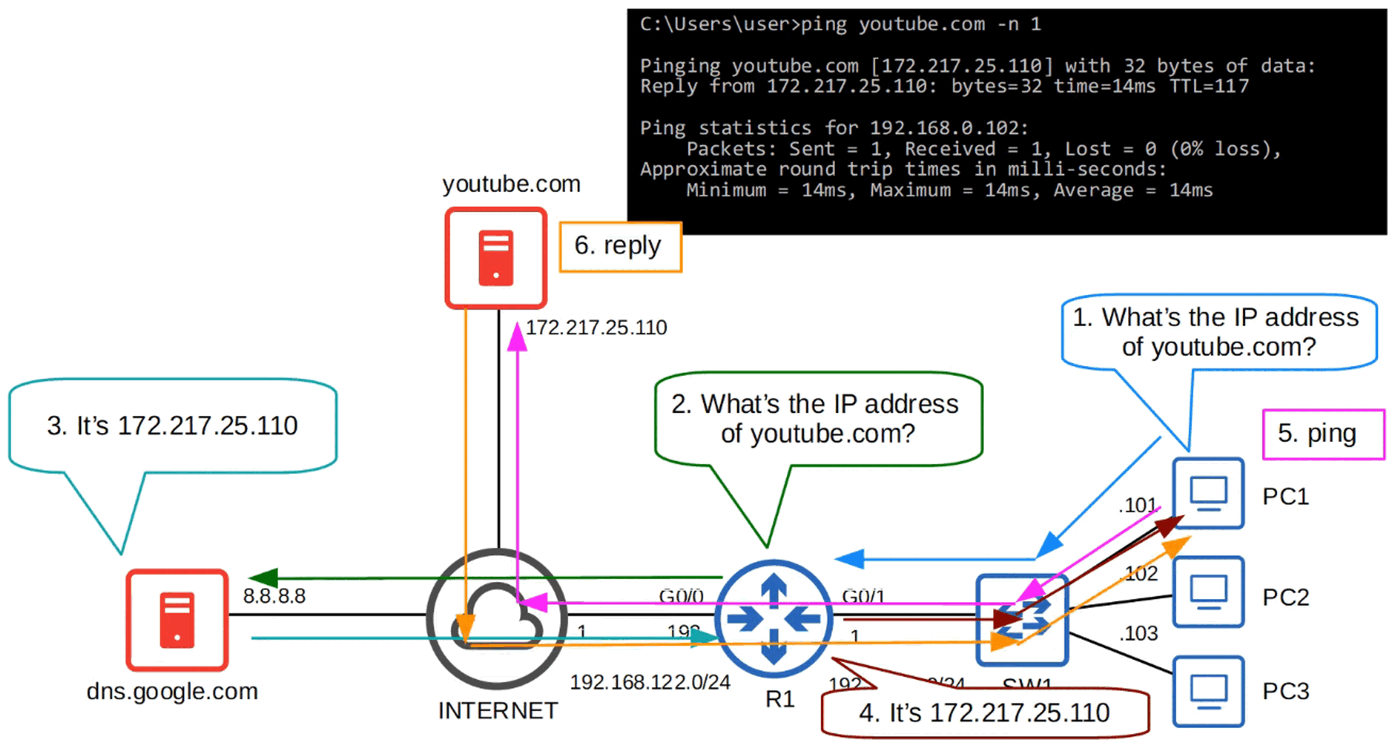
\includegraphics[keepaspectratio,alt={image}]{images/39-dns/img-013.png}}
\end{figure}

Command \passthrough{\lstinline!show hosts!}

\begin{figure}
\centering
\pandocbounded{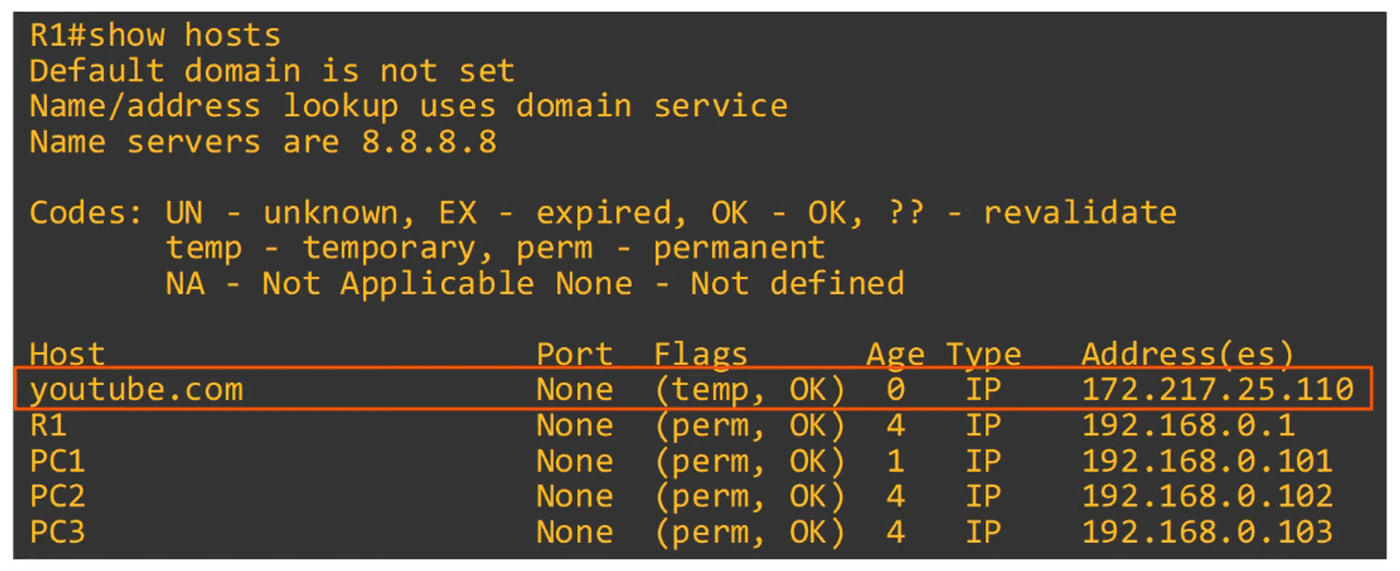
\includegraphics[keepaspectratio,alt={image}]{images/39-dns/img-014.png}}
\end{figure}

Command \passthrough{\lstinline!ip name-server!} and
\passthrough{\lstinline!ip domain lookup!}

\begin{figure}
\centering
\pandocbounded{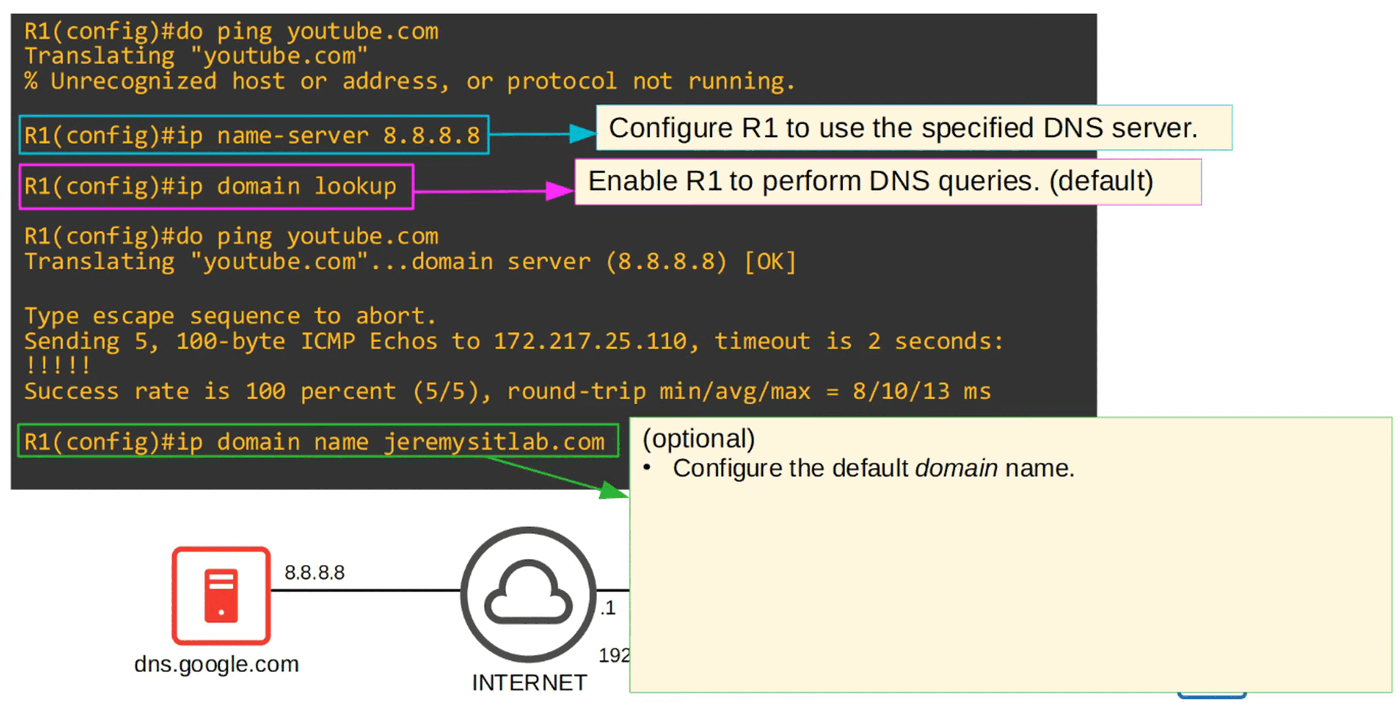
\includegraphics[keepaspectratio,alt={image}]{images/39-dns/img-015.png}}
\end{figure}

\section{Command Review}\label{command-review}

\begin{figure}
\centering
\pandocbounded{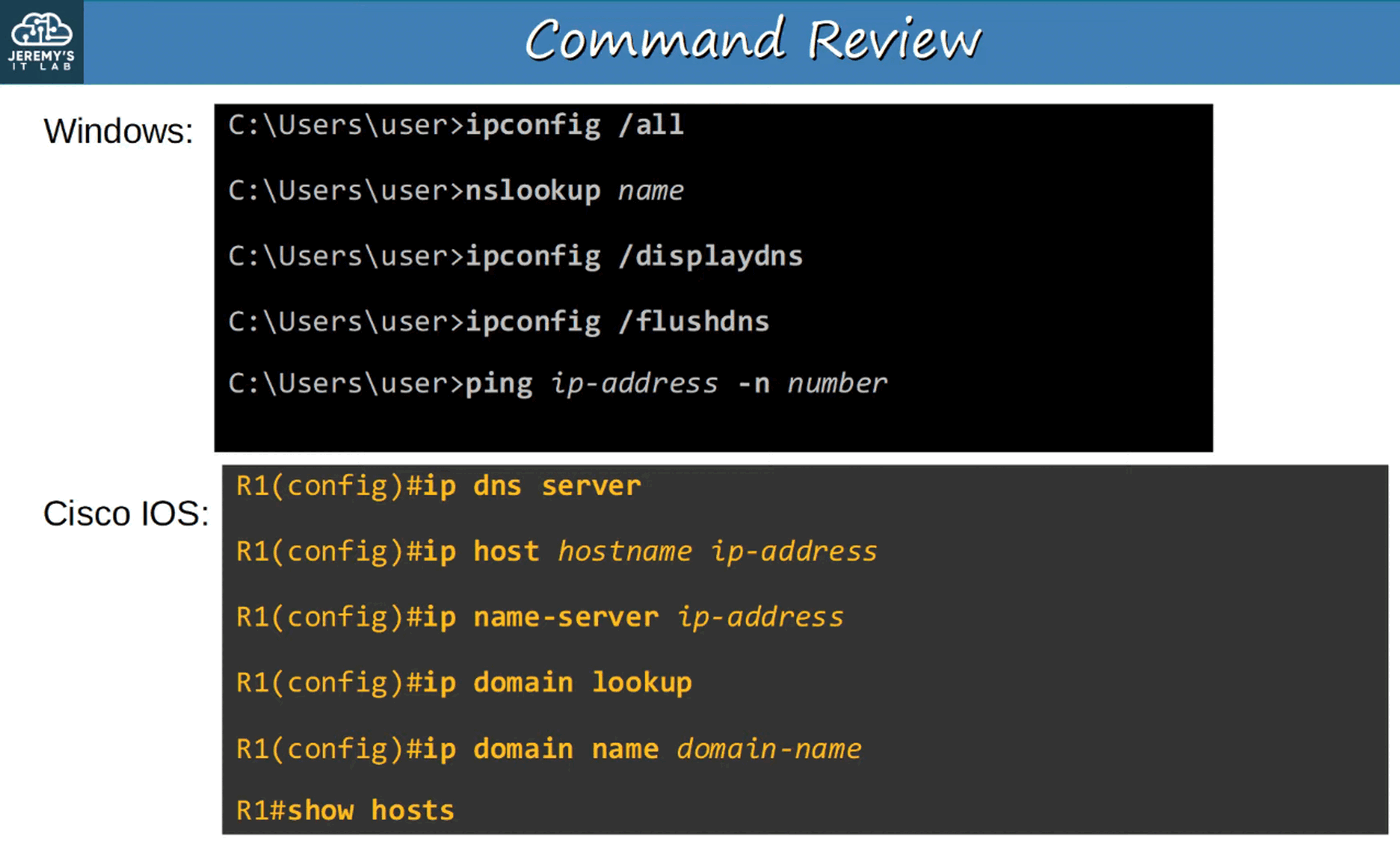
\includegraphics[keepaspectratio,alt={image}]{images/39-dns/img-016.png}}
\end{figure}
